\chapter{Wyniki}
\label{cha:wyniki}

\section{Gry 3-osobowe}
\label{sec:N3nzal}

\paragraph{Równania standardowe}
\label{sec:r_stan}
\begin{wrapfigure}{rh}{0.5\textwidth}
    \centering
    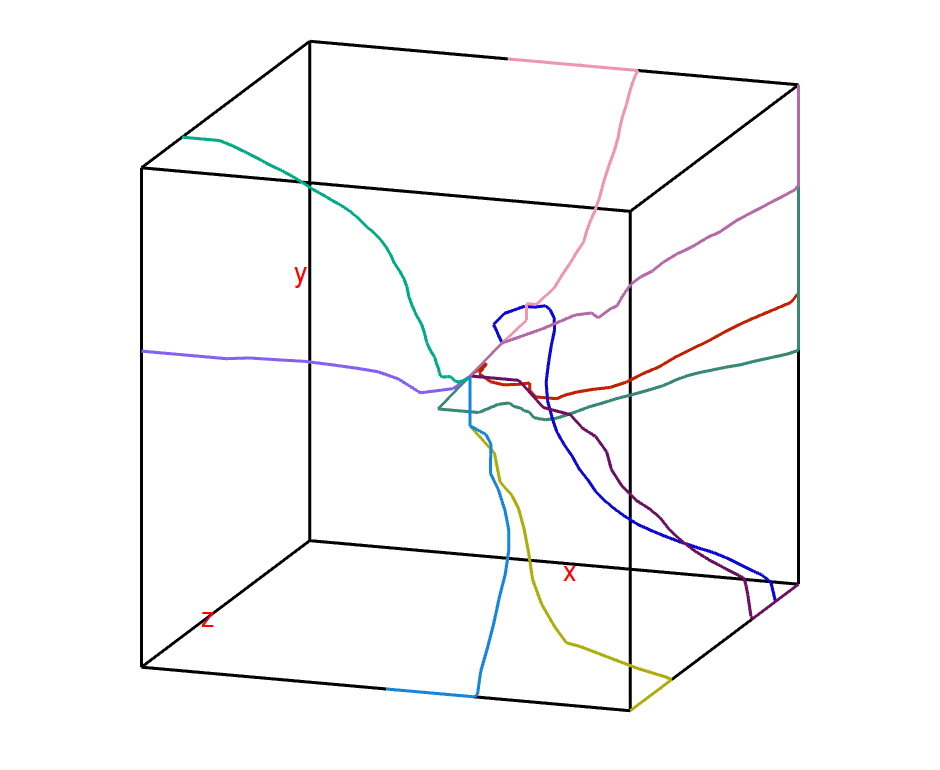
\includegraphics[width=0.5\textwidth]{pict/wyniki/stand100_10.png}   
    \caption{Równania standardowe: 100 gier, 10 graczy}
	\label{fig:stand50_10} 
\end{wrapfigure}

Postaramy się teraz przeanalizować wyniki symulacji z użyciem równań standardowych. Z analizy teoretycznej równań spodziewamy się zawiązania koalicji pomiędzy dwójką z graczy, wynikiem tego jest dążenie funkcji do krawędzi sześcianu. Po osiągnięcia trwałej koalicji trzeci gracz bezskutecznie stara się grać na jednego z koalicjantów. Jest to widoczne poprzez poruszanie się funkcji po krawędzi sześcianu dążącej do jego wierzchołków. Widać że funkcje idące od centrum zachowują się w miarę stabilnie idąc w kierunku jakiejś krawędzi nie zmieniają monotoniczności. Istnieją niewielkie wahania wynikające z prawdopodobieństwa, ale nie mają one większego wpływu w dążeniu do jednej z krawędzi i zmianę ich decyzji. 

Tak naprawdę koalicje zawiązują się tuż po zaczęciu gry i dążą bezpośrednio do stanu ustalonego,  ponieważ na początku gry szacowane prawdopodobieństwo u innych graczy jest bardzo duże. Wynika to z tego szacowane prawdopodobieństwo w pierwszej grze wynosi 0\% albo 100\% co definitywnie wskazuje aby grać na jednego z zawodników. Było to powodem dla którego wprowadziłem współczynnik $\alpha$ równy 0.1, który ma za zadanie blokować sytuacje w których od razu po pierwszej grze jesteśmy w trwałej koalicji.

Jeśli chcielibyśmy uzyskać szybszą grę powinniśmy używać większych współczynników $\alpha$, co skutkować będzie mniejszą szansą na zerwanie koalicji. Jeśli natomiast chcielibyśmy żeby gra przebiegała wolniej moglibyśmy obniżyć współczynnik $\alpha$, co doprowadziłoby do większej liczby zmian partnerów.


%\lipsum[1-5]

%---------------------------------------------------------------------------------------------------------------------------------------------------------
\paragraph{Równania replikatorów}
\label{sec:r_repl}

\begin{figure}
	\centering
	\begin{tabular}{c|c}
		\centering
		\subfloat[50 gier \label{fig:repl100_10}]{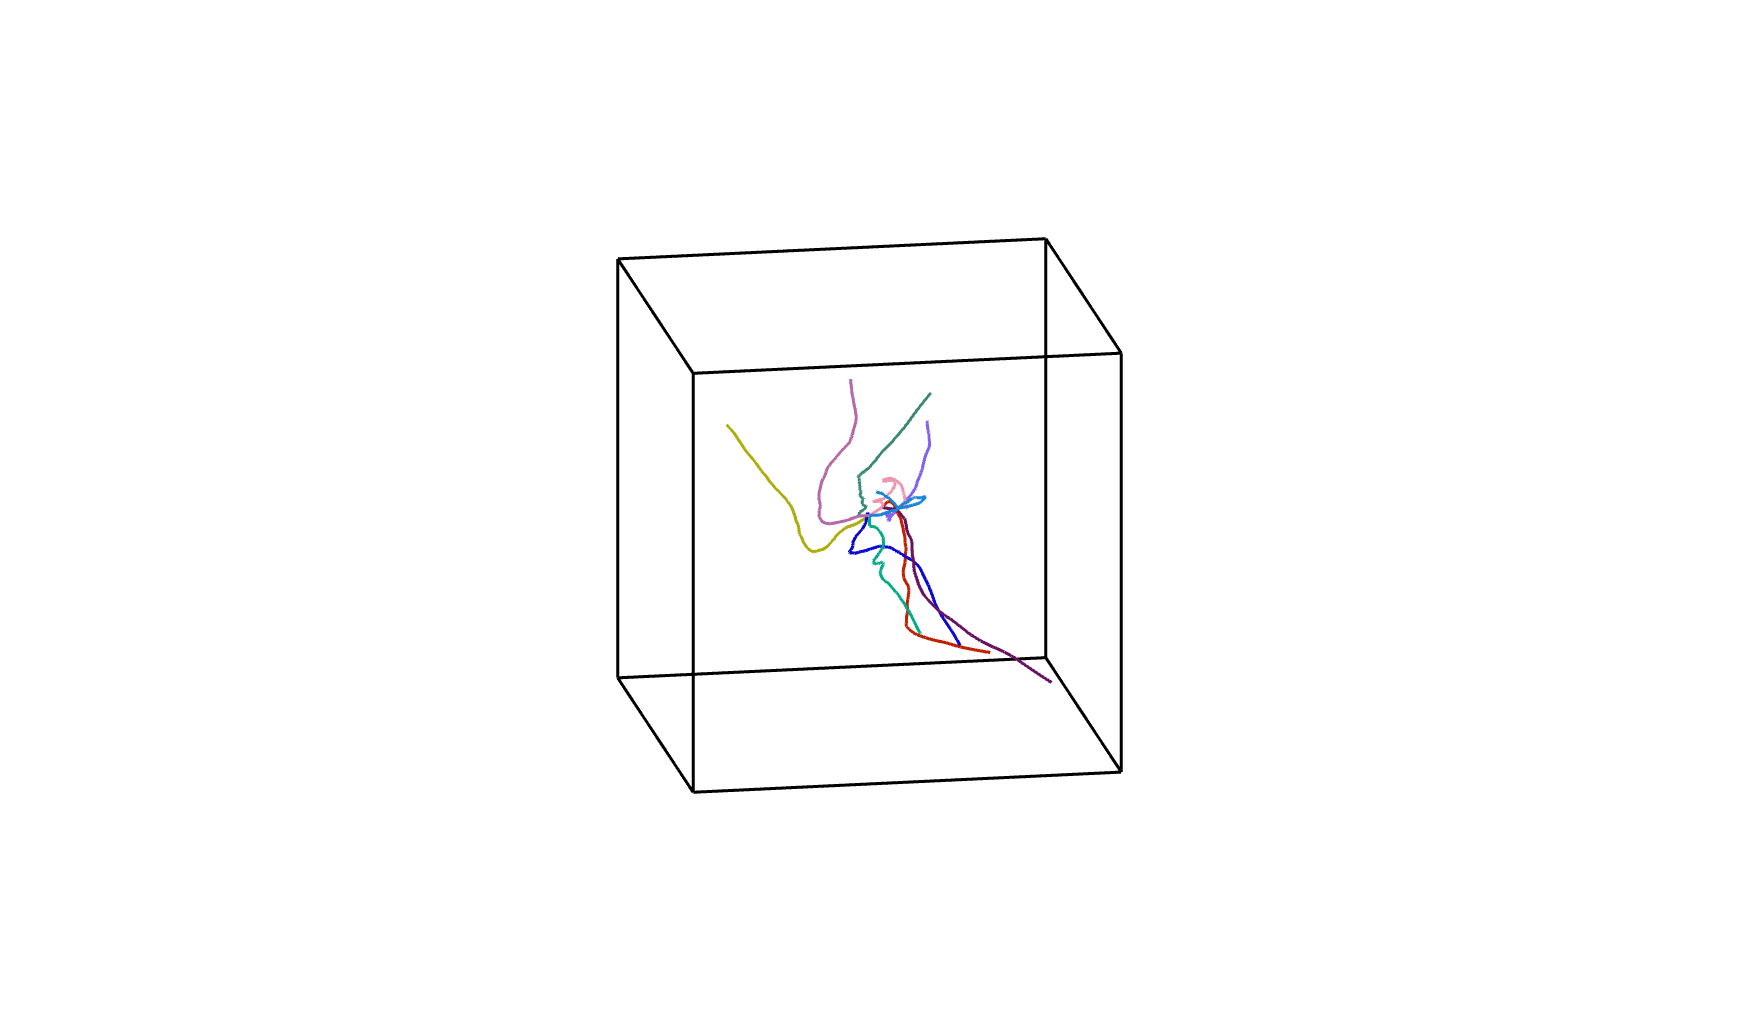
\includegraphics[width=.45\textwidth]{pict/wyniki/repl100_10.png}} 
		&
		\subfloat[250 gier \label{fig:repl250_10}]{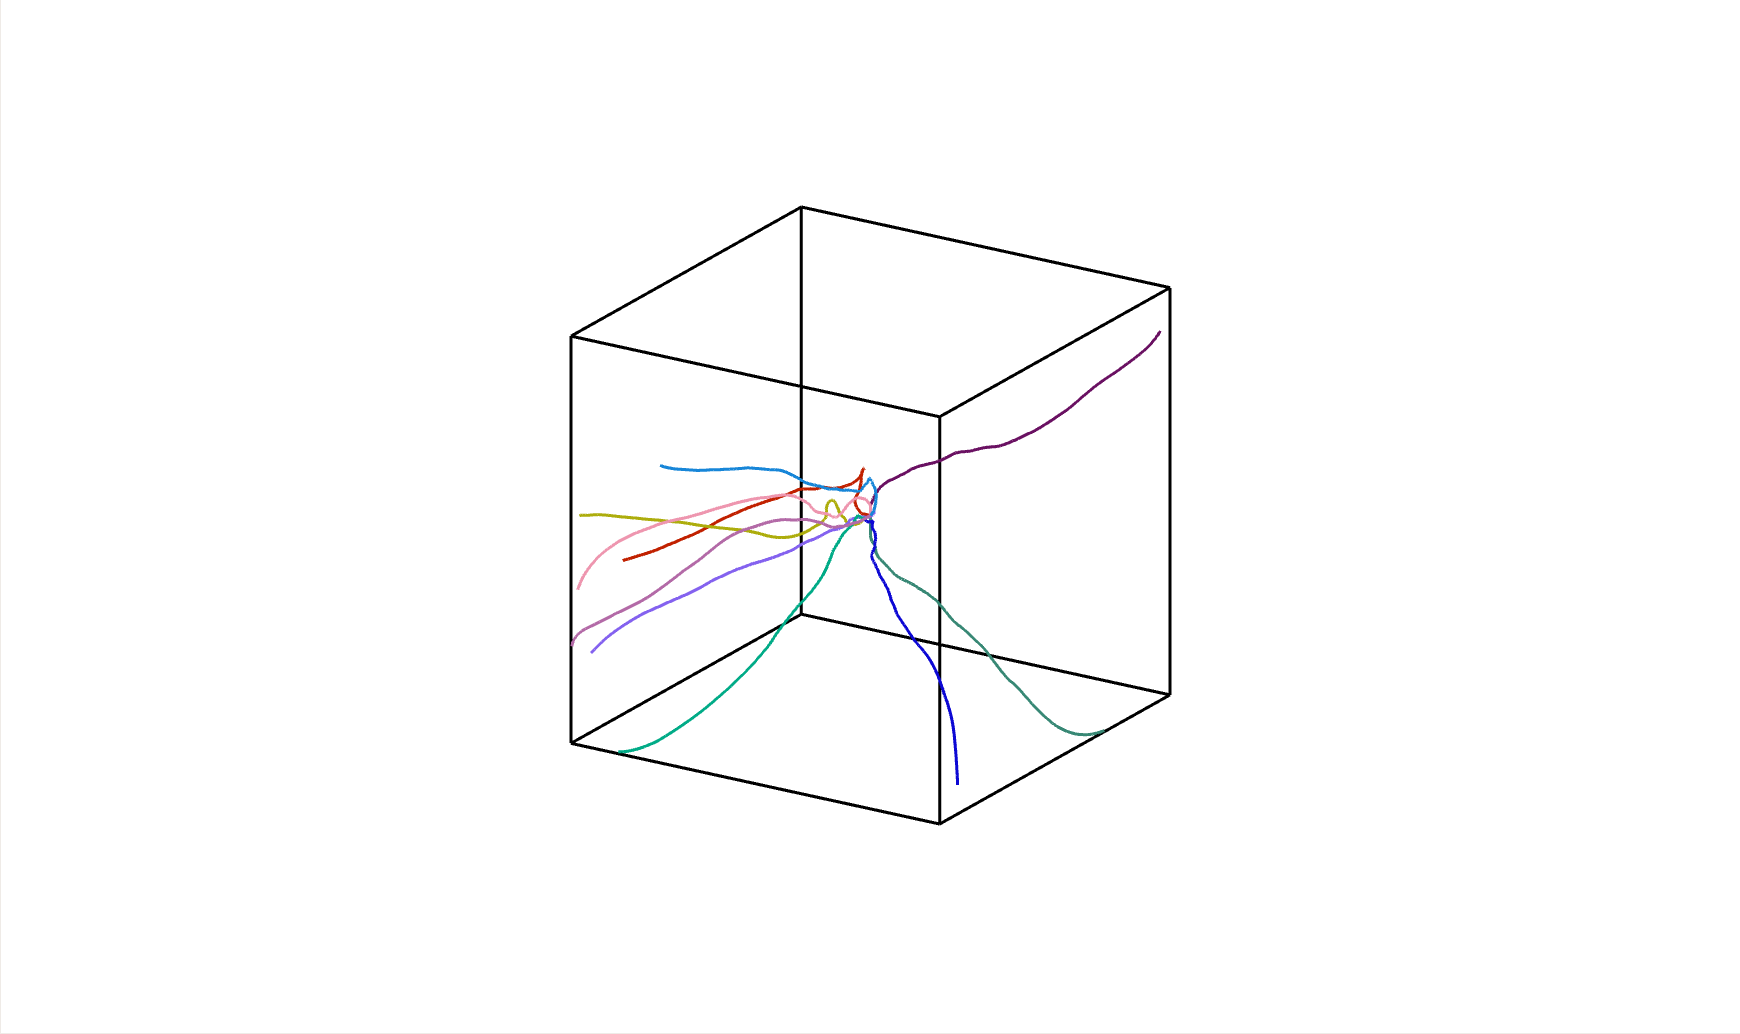
\includegraphics[width=.45\textwidth]{pict/wyniki/repl250_10.png}}
		\\ \hline
		\subfloat[1000 gier \label{fig:repl1000_10}]{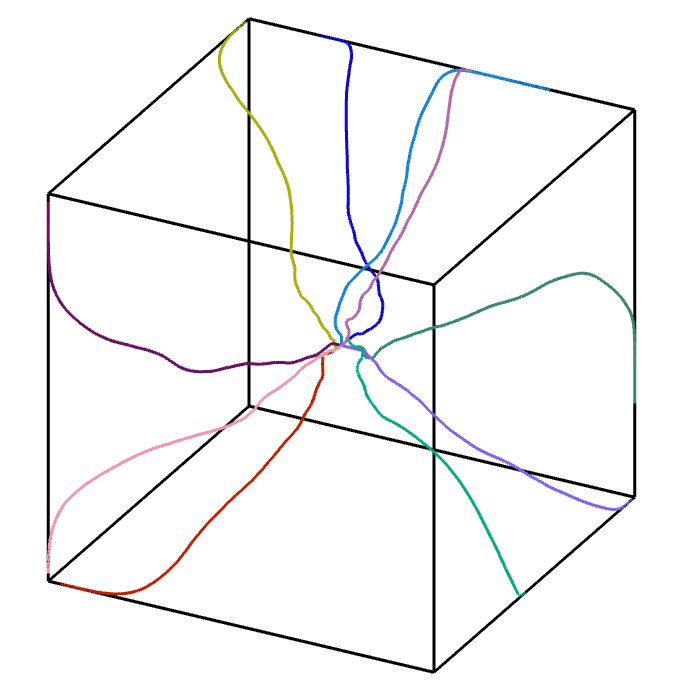
\includegraphics[width=.45\textwidth]{pict/wyniki/repl1000_10.png}}
		&
		\subfloat[10000 gier \label{fig:repl10000_10}]{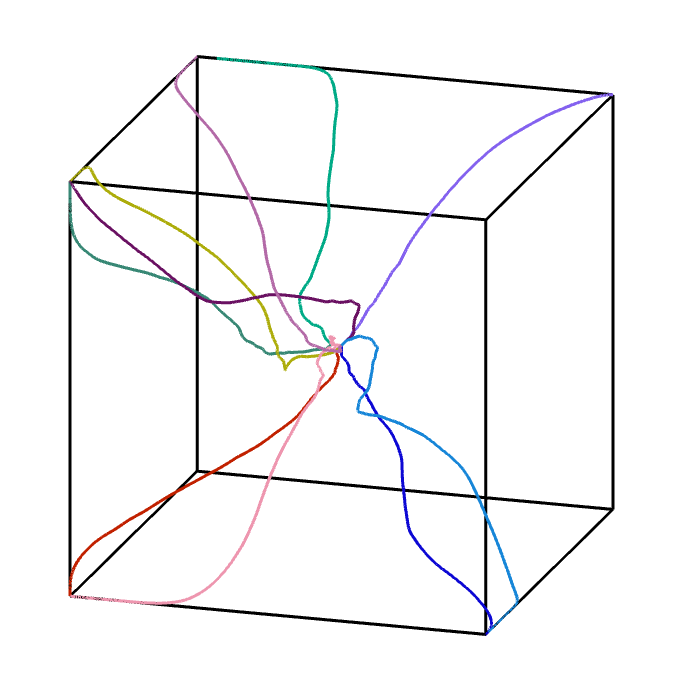
\includegraphics[width=.45\textwidth]{pict/wyniki/repl10000_10.png}}
	\end{tabular}
\caption{Równania replikatorów: 10 graczy}
\label{fig:repl_10}
\end{figure}

Od równania tego rodzaju spodziewamy się mniejszego wkładu, a jest to spowodowane tym że człon z własnym prawdopodobieństwem jest funkcja kwadratową $x(1-x)$ której maksimum ma wartości 0.5 i wynosi ono 0.25. Na krańcach dziedziny funkcji $<0,1>$ przyjmuje wartość 0 (przypomina wielomian węzłowy Lagrange'a). Co jest znacznym ograniczeniem dynamiki funkcji w stosunku do równań standardowych. Dobrym tego przykładem jest rysunek \ref{fig:repl50_10} na którym widać jak dla 50 gier prawdopodobieństwa zachowujemy się dużo wolniej w porównaniu z równaniami standardowymi co jest bezpośrednim wynikiem omawianego członu. Ograniczenie zmiany prawdopodobieństwa wprowadza możliwość zmiany koalicji, ponieważ prawdopodobieństwo przejścia między koalicjami wzrasta ze spadkiem maksymalnej pojedynczej jego zmiany. Widoczne na rysunku \ref{fig:repl50_10} kiedy to w początkowej fazie kilka koalicji rozwiązuje się i zmieniają partnerów, co nie było widoczne dla równań standardowych. Na rysunku \ref{fig:repl250_10} widzimy że tak samo jak dla równania standardowych i w tym przypadku funkcje prawdopodobieństwa dążą do krawędzi sześcianu, jednak dzieje się to znacznie wolniej gdyż człon równania z własnym prawdopodobieństwem dąży do 0. Dopiero dla 1000 gier zaczynamy obserwować sytuację podobną do 50 gier dla równań standardowych kiedy to funkcje prawdopodobieństwa dochodzą do krawędzi sześcianu i jeden z osamotniony graczy za wszelką cenę stara się grać tylko na jednego z partnerów aby wybić go ze stanu równowagi, co prowadzi do zmierzania do wierzchołków sześcianu, gdzie stan ustalony wygląda jako koalicja dwóch graczy z jednym wyobcowanym zawodnikiem, który jest zdecydowany na grę z jednym graczem lecz partner nie odwzajemnia jego chęci. Aż 10000 gier było wymagane aby prawdopodobieństwa doszły do wierzchołka gdzie mamy wcześniej opisaną sytuację.
%\lipsum[1-5]

%---------------------------------------------------------------------------------------------------------------------------------------------------------
\section{Gry N-osobowe}
\label{sec:N3zal}
\begin{wrapfigure}{rh}{0.5\textwidth}
    \centering
    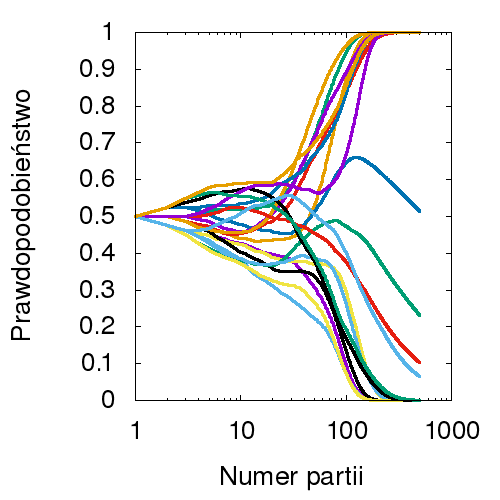
\includegraphics[width=0.5\textwidth]{pict/wyniki/g500p20}   
    \caption{Gra w okręgu: 500 gier, 20 graczy}
	\label{fig:podst} 
\end{wrapfigure}

Chciałbym teraz przeanalizować wyniki jednej z symulacji \ref{fig:podst}. Jak już wcześniej zaobserwowaliśmy równania replikatorów dają dużo mniejszą dynamikę decyzji graczy.

Peleton graczy tworzy stabilne koalicje około 300 partii które nie są w stanie ulec zmianie. Pozostałe przypadki tworzą niestabilne koalicje, które zmieniają się w czasie. Najlepszym tego przykładem jest gracz który początkowo gra w kierunku swojego prawego sąsiada, a później zapewne przez jego niechęć po kilku fluktuacjach zaczyna drastycznie zmieniać partnera swojej gry - zaznaczonych kolorem fioletowym. Czynnik losowy graczy utrudnia grę tylko z jednym wybranym partnerem, dlatego jak widzimy podczas pierwszych 50 gier dochodzi do dużej liczby zmian zachowań graczy. Szczególnie widoczne jest to w pierwszych 50 partiach, gdzie gracze dopiero szacują zachowanie sąsiadów. W kolejnych 50 partiach gracze zachowują się coraz bardziej liniowo, gdyż błąd przewidywanego i realnego prawdopodobieństwa przeciwnika spada. Nie wchodzący w stałą koalicja mogą należeć do łańcucha graczy niezdecydowanych lub jednostek znajdujących się pomiędzy dwoma silnymi koalicjami które nie dają szansy na przyłączenie się do żadnej. Wartym zauważenia jest fakt że ostatnia zmiana monotoniczności funkcji zachodzi dopiero około 300 gry.

\begin{wrapfigure}{rh}{0.5\textwidth}
    \centering
    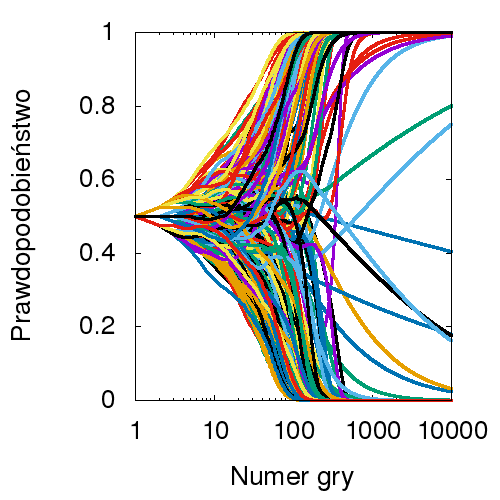
\includegraphics[width=0.5\textwidth]{pict/wyniki/g10000p200}   
    \caption{Gra w okręgu: 10000 gier, 200 graczy}
	\label{fig:niechciani} 
\end{wrapfigure}

Rozpatrzmy teraz dużo dłuższą grę w której zaangażowanych jest więcej graczy, co może pokazać nam przypadki szczególne. Na rysunku widzimy że większość zawodników osiąga stabilne koalicję przed grą 1000. Występuje grupka kilku graczy którzy pomimo tak dużej ilości gier nie byli w stanie zawiązać trwałych koalicji.

Mogło to wynikać z dwóch faktów. Po pierwsze mogli znaleźć się między graczami znajdującymi się w trwały w sojuszach którzy nie byli zainteresowani wchodzeniem w nowe. Drugą przyczyną może być nieznajomość prawdziwego prawdopodobieństwa podejmowania decyzji przez sąsiadów które jest tylko wartością znaną z rozgrywki różnica pomiędzy faktycznym prawdopodobieństwem gry sąsiada a tym co reprezentował. W rozgrywce może się znacząco różnić wpływając na mylną ocenę prawdopodobieństwa gry zawodników i mogących ustalić stabilnej koalicji. Rysunek \ref{fig:niechciani} pokazuje przypadek w którym dwóch silnych koalicjantów nie jest zainteresowanych wejście w sojusz z osamotnionym zawodnikiem między nimi, który jak widać z tabelki !!!REF!!! ZRÓB TABELKĘ !!! powoli próbuje dążyć do stałej koalicji z jednym z graczy.  

